\section{Description}

The following description is based on \textit{\textcolor{blue}{Chapter 8: Numerical Methods, Project 2: Monte Carlo Option Pricing: Pricing Financial Options by Flipping a Coin}} of \cite{mainbook}.

A discrete model for change in price of a stock over a time interval $[0, T]$ is
\begin{equation}
	S_{n+1} = S_n + \mu S_n \Delta t + \sigma S_n \varepsilon_{n+1} \sqrt{\Delta t}, \quad S_0 = s,
	\label{c1:model}
\end{equation}
where $S_n = S(t_n)$ is the stock price at time $t_n = n \Delta t$, $n = 0, \dots, N-1$, $\Delta t = T/N$, $\mu$ is the annual growth rate of the stock, and $\sigma$ is a measure of the stock's annual price volatility or tendency to fluctuate. Highly volatile stocks have large values for $\sigma$, for example, values ranging from 0.2 to 0.4. Each term in the sequence $\varepsilon_1, \varepsilon_2, \dots$ takes on the value 1 or $-1$ depending on whether the outcome of a coin tossing experiment is heads or tails, respectively. Thus, for each $n = 1, 2, \dots$,
\begin{equation}
	\varepsilon_n = 
	\begin{cases} 
		1 & \text{with probability} = \dfrac{1}{2} \\[0.3cm]
		-1 & \text{with probability} = \dfrac{1}{2}.
	\end{cases}
\end{equation}

A sequence of such numbers can easily be created by using one of the random number generators available in most mathematical computer software applications. Given such a sequence, the difference equation \eqref{c1:model} can then be used to simulate a \textbf{sample path} or \textbf{trajectory} of stock prices, $\left\{ s, S_1, S_2, \dots, S_N \right\}$. The ``random'' terms $\sigma S_n \varepsilon_{n+1} \sqrt{\Delta t}$ on the right-hand side of \eqref{c1:model} can be thought of as ``shocks'' or ``disturbances'' that model fluctuations in the stock price. By repeatedly simulating stock price trajectories and computing appropriate averages, it is possible to obtain estimates of the price of a \textbf{European call option}, a type of financial derivative. A statistical simulation algorithm of this type is called a \textbf{Monte Carlo method}.

A European call option is a contract between two parties, a holder and a writer, whereby, for a premium paid to the writer, the holder acquires the right (but not the obligation) to purchase the stock at a future date $T$ (the \textbf{expiration date}) at a price $K$ (the \textbf{strike price}) agreed upon in the contract. If the buyer elects to exercise the option on the expiration date, the writer is obligated to sell the underlying stock to the buyer at the price $K$. Thus the option has, associated with it, a \textbf{payoff function}
\begin{equation}
	f(S) = \max(S - K, 0),
	\label{c1:payoff_func}
\end{equation}
where $S = S(T)$ is the price of the underlying stock at the time $T$ when the option expires (see \figref{c1:f1}).

\begin{figure}[h]
	\begin{center}
		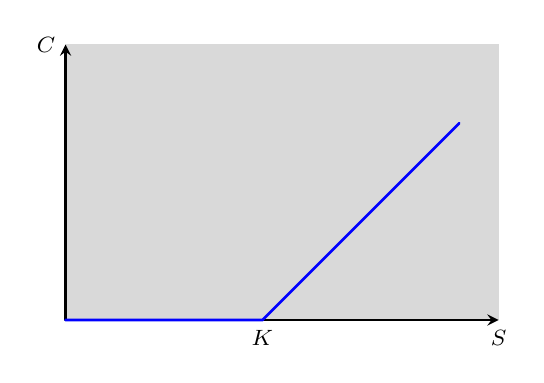
\begin{tikzpicture}[>=stealth,line join=round,line cap=round,font=\footnotesize,scale=0.5]
			\fill[gray,opacity=0.3] (0,0)--(0,7)--(11,7)--(11,0)--cycle;
			
			\draw[->,line width=0.8pt] (0,0)--(0,7) node[left]{$C$};
			\draw[->,line width=0.8pt] (0,0)--(11,0) node[below]{$S$};
			
			\draw[blue,line width=1pt] (0,0)--(5,0) node[below,black]{$K$}--(10,5);
		\end{tikzpicture}
		
		\caption{The value of a call option at expiration is $C = \max(S − K, 0)$, where $K$ is the strike price of the option and $S = S(T)$ is the stock price at expiration.}
		\label{c1:f1}
	\end{center}
\end{figure}

Equation \eqref{c1:payoff_func} is the value of the option at time $T$ since, if $S(T) > K$, the holder can purchase, at price $K$, stock with market value $S(T)$ and thereby make a profit equal to $S(T) - K$, not counting the option premium. If $S(T) < K$, the holder will simply let the option expire since it would be irrational to purchase stock at a price that exceeds the market value. The option valuation problem is to determine the correct and fair price of the option at the time that the holder and writer enter into the contract.\footnote{The 1997 Nobel Prize in Economics was awarded to Robert C. Merton and Myron S. Scholes for their work, along with Fischer Black, in developing the Black--Scholes options pricing model.}

To estimate the price of a call option using a Monte Carlo method, an ensemble
\begin{equation*}
	\left\{ S_N^{(k)} = S^{(k)}(T), \quad k = 1, \dots, M \right\}
\end{equation*}
of $M$ stock prices at expiration is generated using the difference equation
\begin{equation}
	S_{n+1}^{(k)} = S_n^{(k)} + r S_n^{(k)} \Delta t + \sigma S_n^{(k)} \varepsilon_{n+1}^{(k)} \sqrt{\Delta t}, \quad S_0^{(k)} = s.
	\label{c1:estimation}
\end{equation}
For each $k = 1, \dots, M$, the difference equation \eqref{c1:estimation} is identical to equation \eqref{c1:model}, except that the growth rate $\mu$ is replaced by the annual rate of interest $r$ that it costs the writer to borrow money. Option pricing theory requires that the average value of the payoffs $\{f(S_N^{(k)}), k = 1, \dots, M\}$ be equal to the compounded total return obtained by investing the option premium, $\hat{C}(s)$, at rate $r$ over the life of the option,
\begin{equation}
	\frac{1}{M} \sum_{k=1}^M f(S_N^{(k)}) = (1 + r \Delta t)^N \hat{C}(s).
	\label{c1:total}
\end{equation}
Solving \eqref{c1:total} for $\hat{C}(s)$ yields the Monte Carlo estimate
\begin{equation}
	\hat{C}(s) = (1 + r \Delta t)^{-N} \left\{ \frac{1}{M} \sum_{k=1}^M f(S_N^{(k)}) \right\}
	\label{c1:monte_carlo_estimation}
\end{equation}
for the option price. Thus the Monte Carlo estimate $\hat{C}(s)$ is the present value of the average of the payoffs computed using the rules of compound interest.